% Copyright (C) 2005-2015 Airbus - EDF - IMACS - Phimeca
% Permission is granted to copy, distribute and/or modify this document
% under the terms of the GNU Free Documentation License, Version 1.2
% or any later version published by the Free Software Foundation;
% with no Invariant Sections, no Front-Cover Texts, and no Back-Cover
% Texts.  A copy of the license is included in the section entitled "GNU
% Free Documentation License".
\renewcommand{\filename}{docUC_CentralUncertainty_CobWebGraph}
\renewcommand{\filetitle}{UC : Sensitivity analysis : Cobweb graph}

% \HeaderNNIILevel
% \HeaderIILevel
\HeaderIIILevel


\index{Sensitivity Analysis!Cobweb graph}


The Cobweb graph enables to visualize all the combination of the input variables which lead to a specific range of the output variable.\\

Let's suppose a model $f : \Rset^n \longrightarrow  \Rset$, where $f(\vect{X}) = Y$.\\

The graph requires to have a numerical sample \textit{inputSample} of $\vect{X}$ and the output sample of $Y$ defined as :
\begin{align*}
  outputSample = f(inputSample)
\end{align*}

Figure (\ref{CobWeb}) draws such a graph : each column represents one component $X_i$ of the input vector $\vect{X}$. The last column represents the scalar output variable $Y$.  \\
For each point $\vect{X}^j$ of \textit{inputSample}, each component $X_i^j$ is noted on its respective axe and the last mark is the one which corresponds to the associated $Y^j$. A line joins all the marks. Thus, each point of the sample corresponds to a particular line on the graph.\\

The scale of the axes are quantile based :  each axe runs between 0 and 1 and each value is represented by its quantile with respect to its marginal empirical distribution.\\

It is interesting to select, among those lines, the ones which correspond to a specific range of the output variable. These particular lines are colored differently. This specific range is defined in the quantile based scale of $Y$ or in its specific scale. In that second case, the range is automatically converted into a quantile based scale range.\\

\begin{figure}[H]
  \begin{center}
    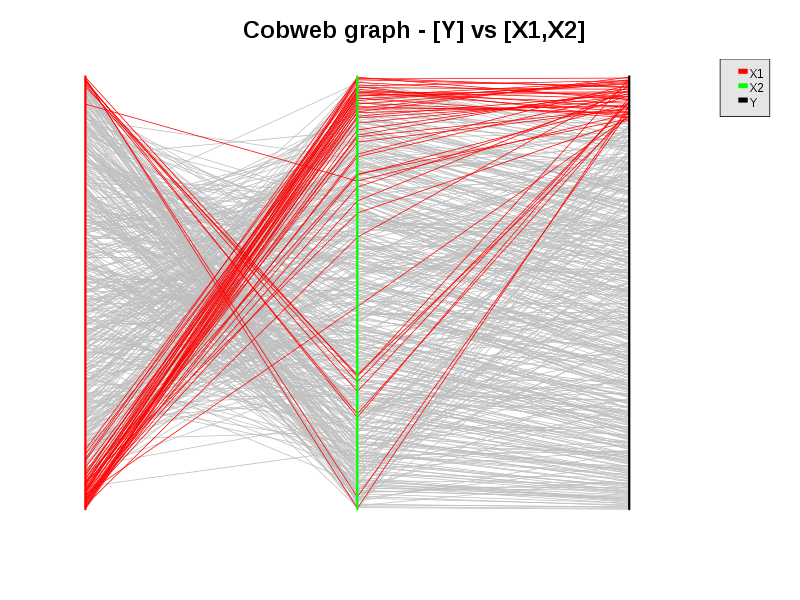
\includegraphics[width=8cm]{Figures/cobWeb.png}
    \caption{The CobWeb graph : a graphical sensitivity analysis tool}
    \label{CobWeb}
  \end{center}
\end{figure}


Figure (\ref{CobWeb}) has been obtained for the following example. The model is
\begin{align*}
  f : \Rset^2 \longrightarrow  \Rset
\end{align*}
where
\begin{align*}
  y = f(x_1, x_2)  = x_1^2 + x_2
\end{align*}
The input random vector $\vect{X}$ follows a bidimensional Normal distribution with $\vect{0}$ mean, a reduced standard deviation vector and a correlation factor $\rho = -0.6$.\\
A numerical sample of $\vect{X}$ of size 500 has been generated and the associated output values have been evaluated.\\
The red curves are the lines where the output variable is in the range $[0.9, 1]$ in the rank based scale.\\
We conclude that the high value of $Y$ are mainly obtained for low values of $X_1$ and high values for $X_2$.\\


\requirements{
  \begin{description}
  \item[$\bullet$] the input sample {\em inputSample}
  \item[type:] a NumericalSample
  \item[$\bullet$] the corresponding output sample {\em outputSample}
  \item[type:] a NumericalSample
  \end{description}
}
             {
               \begin{description}
               \item[$\bullet$] the Cobweb graph
               \item[type:] a Graph
               \end{description}
             }

             \textspace\\

             Python  script for this UseCase :

             \inputscript{script_docUC_CentralUncertainty_CobWebGraph}
